\subsection{Where the error concentrates}
\label{sec:onde_erro}

The per-event 3-D error falls with the detected light: the Spearman rank correlation $\rho_{\mathrm{S}}$ is \num{-0.68} for GATv2-cascade and \num{-0.72} for XGBoost on clean light. By test-light quartile (boundaries: \num{201}, \num{387} and \qty{773}{\pe}), the mean 3-D error of GATv2-cascade is \num{42.79}, \num{31.25}, \num{18.19} and \qty{11.67}{\cm}, and that of XGBoost is \num{47.28}, \num{35.74}, \num{20.78} and \qty{6.98}{\cm} (Figure~\ref{fig:erro_luz}): GATv2-cascade errs less in the three dimmest quartiles (paired differences with intervals above zero), and XGBoost errs less in the brightest, by \qty{4.70}{\cm} (\num{3.58} to \qty{5.75}{\cm}). The centroids with quadratic and linear weights account for \num{43.5} and \qty{33.3}{\percent}, respectively, of the gain importance of XGBoost, trained on augmented light. Since both become more precise with more light, this is consistent with the advantage of XGBoost in the bright events but does not explain it: GATv2-cascade receives the same two centroids among the event-level scalars (Section~\ref{sec:dados_grafos}), and the cause of its larger error in these events was not investigated.

In the sensor frame, the $y$ axis, normal to the long walls, has the lowest RMSE for GATv2-cascade (\qty{14.35}{\cm}, against \num{20.45} and \qty{20.46}{\cm} in $x$ and $z$), for GPS, for the boosters on clean light and for the network of the previous stage (axes converted by an inferred correspondence; Table~\ref{tab:referencias}). The $x$ axis, normal to the faces without channels, has the highest for the boosters (XGBoost: \qty{23.82}{\cm}) and for that network (\qty{24.68}{\cm}). The coefficient of determination $R^2$ of GATv2-cascade in $z$, the fraction of the variance explained, is \num{0.9994} because the standard deviation of the test vertices is \num{4.6} times as large in $z$ as in $x$, not because $z$ is better reconstructed.

Below $z = {}$\qty{20}{\m} (\num{626} events), the RMSE values in $z$ of the calibrated barycentre, of GATv2-cascade and of XGBoost on clean light are close to one another (\num{23.29}, \num{22.54} and \qty{22.63}{\cm}); from \qty{20}{\m} upwards (\num{311} events), that of the barycentre rises to \qty{65.87}{\cm}, and the other two fall to \num{15.44} and \qty{18.91}{\cm} (Figure~\ref{fig:erro_z}). The factor \num{2.07} of Section~\ref{sec:comparacao_referencias} comes from these vertices: the channels of the end cap, all at $z = {}$\qty{29.93}{\m}, receive \qty{41.2}{\percent} of the light and shift the barycentre all the more the further the vertex lies from the long walls, which the calibration, a function of $\bar{z}$ alone, does not correct.

\begin{figure}[H]
  \centering
  \begin{subfigure}[t]{0.485\textwidth}
    \centering
    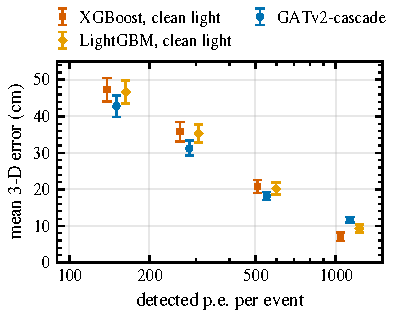
\includegraphics{figures/erro_luz.pdf}
    \caption{Mean 3-D error of GATv2-cascade and, on clean light, of \mbox{XGBoost} and \mbox{LightGBM}, by quartile of the detected light in the \num{937} test events; points at the mean light of the quartile, those of the boosters offset sideways, and \qty{95}{\percent} bars on each mean, from a bootstrap over the events of the quartile. GATv2-cascade errs less in the three dimmest quartiles, and \mbox{XGBoost} in the brightest (\qty{773}{\pe} or more); the interval of the paired difference between the two excludes zero in every quartile.}
    \label{fig:erro_luz}
  \end{subfigure}\hfill
  \begin{subfigure}[t]{0.485\textwidth}
    \centering
    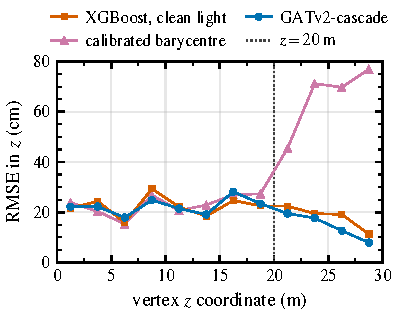
\includegraphics{figures/erro_z.pdf}
    \caption{RMSE in $z$ of GATv2-cascade, of the calibrated barycentre and of \mbox{XGBoost} on clean light in the test events, per \qty{2.5}{\m} bin of the vertex $z$; dotted line at \qty{20}{\m}. Up to \qty{20}{\m}, the errors are close to one another; near the end cap ($z = {}$\qty{29.93}{\m}), that of the barycentre rises and that of GATv2-cascade falls.}
    \label{fig:erro_z}
  \end{subfigure}
  \caption{Where the error concentrates in the test events: (a)~by quartile of detected light; (b)~by bin of the vertex $z$.}
  \label{fig:par_onde_erro}
\end{figure}
